% Section 3. Principal evidence on vehicle-currency formation.
% Displayed quantities bind to generated exhibits under output/.

\section{How stablecoins gain the vehicle role}
\label{sec:dominance}

\subsection{The aggregate rotation}
\label{sec:dominance:transition}

Stablecoins carry a much larger share of vehicle activity in 2026 than in 2024. The comparison uses the same January--June dates in both years because the 2026 panel ends on June 30. Giving each matched day equal weight, stablecoins' share among native and stable intermediaries rises from \StableCountBase{} to \StableCountEnd{} by route count and from \StableValueBase{} to \StableValueEnd{} by routed value. Appendix Table~\ref{tab:app:rotation} reports the paired-day estimates and their sampling uncertainty. The decomposition below pools route activity so its components allocate the aggregate count or value exactly.
% output/exhibits/intermediation_complexity_rival.jsonl; output/exhibits/presentation_values.tex

The half-year series in Figure~\ref{fig:vehicle-composition} reverses direction. Native assets regain share in 2023 and 2024; stablecoins recover the routed-value lead in 2025. The 20\% value-agreement sample covers 71.6\% of native intermediary value and 55.1\% of stablecoin intermediary value in 2026. Fiat-reserve tokens account for \BackingFiatCountChange{} of the \BackingPooledCountChange{} count increase and \BackingFiatValueChange{} of the \BackingPooledValueChange{} value increase. The aggregate movement is therefore mainly a shift toward reserve-backed dollar tokens, although USDT and USDC follow distinct paths in the token-level results below.
% output/exhibits/intermediation_by_type.jsonl; output/exhibits/e0_vehicle_transition_backing_regime_estimates.jsonl

\begin{figure}[tbp]
\centering
\caption{Intermediary activity rotates between native assets and stablecoins}
\label{fig:vehicle-composition}
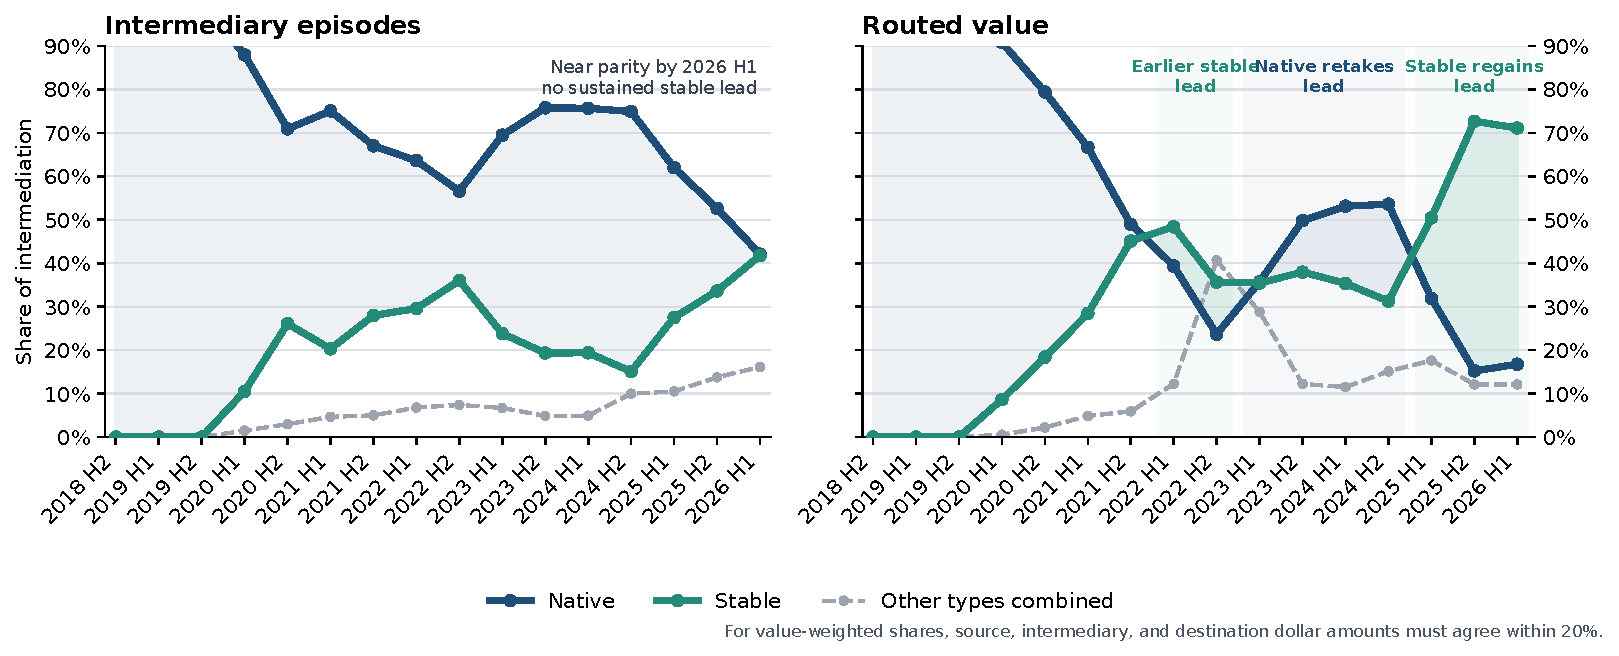
\includegraphics[width=0.98\textwidth]{../output/figures/experiments/annual_vehicle_composition_bands.pdf}
\exhibitnote{The sample contains complete routes that do not return to their starting asset. Each route contributes once for every intermediary it uses, so routes with more than two legs can contribute several observations. Shares are formed across all intermediary types; Appendix Table~\ref{tab:app:rotation} uses the narrower native-or-stable denominator. Every point covers six calendar months; the final point is 2026 H1. Routed value requires source, intermediary, and destination dollar amounts to agree within 20\%.}
\end{figure}

\subsection{Pair formation and persistence}
\label{sec:dominance:pairs}

Aggregate dominance can change inside continuing pairs or through the distribution of activity across pairs. Let $p$ denote a pair and $y\in\{2024,2026\}$. A continuing pair carries native-or-stable routes in both matched periods; a year-specific pair carries them in only one. First split total activity between these two sets. Within continuing pairs, stablecoin share can change because a given pair changes its vehicle mix or because trading shifts toward pairs with a different vehicle mix. The remaining change comes from the aggregate weight on continuing pairs and the stablecoin share of pairs observed in only one period.

Formally, let $W_y$ be the share of native-plus-stable activity in continuing pairs, $\omega_{p,y}$ pair $p$'s weight within that activity, and $s_{p,y}$ its stablecoin share. Continuing pairs have stablecoin share $S_{C,y}=\sum_p\omega_{p,y}s_{p,y}$, while year-specific pairs have share $S_{E,y}$. Total stablecoin share is therefore $S_y=W_yS_{C,y}+(1-W_y)S_{E,y}$. Writing $\Delta x=x_{2026}-x_{2024}$ and $\bar{x}=(x_{2024}+x_{2026})/2$ gives the exact midpoint decomposition
\begin{equation}
\label{eq:pair-decomposition}
\begin{aligned}
\Delta S={}&
\underbrace{\bar{W}\sum_p\bar{\omega}_p\Delta s_p}_{\text{switching within continuing pairs}}
+\underbrace{\bar{W}\sum_p\bar{s}_p\Delta\omega_p}_{\text{activity shifting across pairs}}\\
&+\underbrace{(\bar{S}_C-\bar{S}_E)\Delta W}_{\text{continuing-pair weight}}
+\underbrace{(1-\bar{W})\Delta S_E}_{\text{year-specific pairs}}.
\end{aligned}
\end{equation}

The midpoint averages hold the companion quantity fixed while each component changes, so the four terms add exactly to the aggregate change. The first two terms split the change among continuing pairs into changes in each pair's stablecoin share and changes in pair weights. The last two terms separate the changing mass of continuing pairs from the stablecoin share among period-specific pairs. The two sets partition each period's activity; nothing is deducted from a continuing pair.

We also compare the same pair, date within the year, and realised single- or cross-exchange route class. For route-count or routed-value stablecoin share $S^{(m)}_{pds,y}$, the matched regression is
\begin{equation}
\label{eq:pair-fe}
S^{(m)}_{pds,y}=\alpha^{(m)}_{pds}+\beta^{(m)}\mathbf{1}_{\{y=2026\}}+\varepsilon^{(m)}_{pds,y},
\qquad m\in\{N,V\}.
\end{equation}
Here $d$ is the month-day and $s$ the realised route class. Observations are weighted by native-plus-stable route count or supported routed value; standard errors cluster by pair and date. The comparison is descriptive because route class and trading activity can respond to the same forces as vehicle choice.

Table~\ref{tab:pair-composition} applies Equation~\eqref{eq:pair-decomposition} to route counts and supported value and reports Equation~\eqref{eq:pair-fe} on cells defined by pair, calendar date, and route class.

\FloatBarrier
\begin{table}[tbp]
\centering
\caption{Decomposition of the stablecoin rotation}
\label{tab:pair-composition}
\small
\begin{tabularx}{\linewidth}{@{}>{\raggedright\arraybackslash}Xrr@{}}
\toprule
Component or estimate & Estimate [pp] & Obs. \\
\midrule
\multicolumn{3}{l}{\emph{Panel A. Route-count share: continuing and year-specific pairs}} \\
Net stablecoin-share change within continuing pairs & $-0.1$ & \\
\quad Pairs moving toward stablecoins (1,569) & $+1.3$ & \\
\quad Pairs moving toward native assets (1,487) & $-1.4$ & \\
Vehicle activity shifting across continuing pairs & $+8.4$ & \\
Weight of continuing versus year-specific pairs & $-0.5$ & \\
Net contribution of period-specific vehicle activity & $+17.79$ & \\
\quad Pairs first observed after 2024 H1 & $+20.09$ & \\
\quad Pairs reactivated after absence in 2024 H1 & $+0.20$ & \\
\quad Vehicle-role turnover in continuing pairs & $-0.77$ & \\
\quad Pairs exiting before 2026 H1 & $-1.73$ & \\
\midrule
Total route-count change & $+25.5$ & \\
\addlinespace
\multicolumn{3}{l}{\emph{Panel B. Dollar-weighted share: continuing and year-specific pairs}} \\
Net stablecoin-share change within continuing pairs & $0.0$ & \\
\quad Pairs moving toward stablecoins (1,505) & $+2.3$ & \\
\quad Pairs moving toward native assets (1,445) & $-2.4$ & \\
Vehicle activity shifting across continuing pairs & $+26.2$ & \\
Weight of continuing versus year-specific pairs & $-2.5$ & \\
Net contribution of period-specific vehicle activity & $+19.16$ & \\
\quad Pairs first observed after 2024 H1 & $+21.94$ & \\
\quad Pairs reactivated after absence in 2024 H1 & $+0.04$ & \\
\quad Vehicle-role turnover in continuing pairs & $-1.72$ & \\
\quad Pairs exiting before 2026 H1 & $-1.10$ & \\
\midrule
Total change in dollar-weighted share & $+42.8$ & \\
\addlinespace
\multicolumn{3}{l}{\emph{Panel C. Matched pair estimates}} \\
\midrule
All two-leg routes, count share & $+0.23\ (0.77)$ & 188,344 \\
20\% agreement sample, count share & $+0.32\ (0.75)$ & 182,734 \\
20\% agreement sample, dollar-weighted share & $-1.35\ (2.19)$ & 182,734 \\
\bottomrule
\end{tabularx}

\exhibitnote{Panels A through C compare pooled activity over matched January--June dates in 2024 and 2026. Panels B and C report Equation~\eqref{eq:pair-decomposition}; their indented rows split the within-pair component into positive and negative contributions. Panel C weights routes by dollar value and applies the 20\% agreement rule. Panel D estimates Equation~\eqref{eq:pair-fe}; standard errors use two-way clustering by pair and date. Panels A and B factor the same route-count change in different ways, so their components should not be combined.}
\end{table}

Pooling route counts gives an increase from \PairPooledBase{} to \PairPooledEnd{}, or \PairPooledTotal{}, close to the equal-day change in Appendix Table~\ref{tab:app:rotation}. The within-pair component is \PairPooledWithin{} by route count and \PairValueWithin{} by routed value. These net estimates combine \MarginWithinGrossUp{} from pairs moving toward stablecoins and \MarginWithinGrossDown{} from pairs moving toward the native asset. Activity shifting across continuing pairs contributes \PairPooledReweight{} by count and \PairValueReweight{} by value. The changing aggregate weight on continuing pairs contributes \PairPooledSupportMass{} and \PairValueSupportMass{}, while year-specific pairs contribute \PairPooledExclusive{} and \PairValueExclusive{}. The last component is net of entry and exit: pairs observed only in 2026 add their later-period vehicle use, while pairs observed only in 2024 remove their earlier-period vehicle use. Equation~\eqref{eq:pair-fe} reaches the same conclusion on the more restrictive matched sample: stablecoin share changes by \MatchedMarketCountChange{} by count and \MatchedMarketValueChange{} by value. A large aggregate rotation therefore coexists with little net switching inside established cells defined by pair, calendar date, and route class.
% output/exhibits/vehicle_transition_pair_decomposition.jsonl; output/exhibits/vehicle_transition_pair_fixed_effects.jsonl

The same decomposition covers every adjacent January--June comparison between 2019 and 2026. As shown in Appendix Table~\ref{tab:app:rotation-boundaries}, panel A, the within-pair term ranges only from \AdjacentWithinMin{} to \AdjacentWithinMax{}, while aggregate changes range from \AdjacentLargestDecline{} in \AdjacentLargestDeclineYears{} to \AdjacentLargestIncrease{} in \AdjacentLargestIncreaseYears{}. Pair composition therefore accounts for both stablecoin gains and the intervening reversals.
% output/exhibits/vehicle_transition_adjacent_year_decomposition.jsonl; output/exhibits/result_resolution_values.tex

Endpoint demand clarifies the composition result. A pair with WETH at one endpoint cannot also use WETH as its intermediary, so part of the native-versus-stable allocation is mechanically fixed. Panel A of Appendix Table~\ref{tab:app:endpoint-direction} splits the headline daily change by endpoint direction. Pairs with one native and one stable endpoint contribute \EndpointNativeStableCountContribution{} by route count and \EndpointNativeStableValueContribution{} by routed value; pairs with two stable endpoints contribute \EndpointStableStableCountContribution{} and \EndpointStableStableValueContribution{}, respectively. All other pairs remain the largest channel overall. Panel B shows that USDT supplies \StableStableUsdtValueContribution{} of the two-stable-endpoint value increase, while USDC, DAI, and the remaining stablecoin intermediaries jointly contribute \StableStableOtherValueContribution{}. The result is present on all \StableStableActiveDays{} common days, and trimming the largest decile of daily contributions leaves a \StableStableTrimmedValueChange{} increase. Stablecoin dominance therefore spreads beyond pairs whose endpoint identity limits the native vehicle, while routing between stable currencies concentrates on one intermediary issuer.
% output/exhibits/vehicle_transition_pair_contributions.parquet; output/exhibits/vehicle_transition_pair_decomposition_deck_values.tex; output/exhibits/endpoint_direction_decomposition.jsonl; output/exhibits/endpoint_direction_deck_values.tex; output/exhibits/stable_stable_vehicle_decomposition.jsonl; output/exhibits/stable_stable_vehicle_robustness.jsonl; output/exhibits/stable_stable_vehicle_values.tex

Panel B of Appendix Table~\ref{tab:app:rotation-boundaries} removes every pair with WETH or a stablecoin at either endpoint. Stablecoin vehicle share still rises from \NonvehicleEndpointStableBase{} to \NonvehicleEndpointStableEnd{} by count and from \NonvehicleEndpointValueBase{} to \NonvehicleEndpointValueEnd{} by supported value. Pair entry and exit contribute \NonvehicleEndpointCountExclusive{} and \NonvehicleEndpointValueExclusive{}, respectively. The rotation therefore remains economically large among pairs for which both broad vehicle families are distinct from the assets being exchanged.
% output/exhibits/vehicle_transition_nonvehicle_endpoint_decomposition.jsonl; output/exhibits/result_resolution_values.tex

The first routes in a new pair predict its subsequent vehicle. For pair $p$, let $E_p$ be the stablecoin share on its entry day. For each of the disjoint windows $h\in\{1\text{--}30,31\text{--}120\}$, let $R_{p,h}$ indicate that the pair carries another native- or stablecoin-intermediated route, and let $S_{p,h}$ be the stablecoin share when $R_{p,h}=1$. We estimate
\begin{equation}
\label{eq:entry-persistence}
\begin{aligned}
S_{p,h}&=\alpha_h+\beta_h E_p+X_p'\delta_h+\varepsilon_{p,h},
&& R_{p,h}=1,\\
R_{p,h}&=a_h+b_h E_p+X_p'c_h+u_{p,h},
&& \text{all entrant pairs}.
\end{aligned}
\end{equation}
The second line is a linear probability model. The controls $X_p$ contain the cohort year, a stablecoin-endpoint indicator, log entry-day route count, direct-route share, and complex-route share. The sample uses pairs entering by March 2 in 2024 or 2026, giving every pair 120 complete calendar days of follow-up. Pairs with a native asset at either endpoint are excluded.

\FloatBarrier
\begin{table}[tbp]
\centering
\caption{Vehicle persistence after pair entry}
\label{tab:entry-persistence}
{\tiny
\renewcommand{\arraystretch}{0.90}
\begin{tabularx}{\linewidth}{@{}>{\hsize=1.6\hsize\raggedright\arraybackslash}X*{6}{>{\hsize=.9\hsize\centering\arraybackslash}X}@{}}
\toprule
\multicolumn{7}{@{}l}{\textit{Panel A. Stablecoin route share among pairs that trade again [\%]}} \\
 & \multicolumn{3}{c}{Days 1--30} & \multicolumn{3}{c}{Days 31--120} \\
\cmidrule(lr){2-4}\cmidrule(l){5-7}
 & (1) & (2) & (3) & (4) & (5) & (6) \\
\midrule
Entry stablecoin share [10 pp] & \begin{tabular}{@{}c@{}}$+9.00^{***}$\\$(0.14)$\end{tabular} & \begin{tabular}{@{}c@{}}$+8.92^{***}$\\$(0.15)$\end{tabular} & \begin{tabular}{@{}c@{}}$+8.55^{***}$\\$(0.72)$\end{tabular} & \begin{tabular}{@{}c@{}}$+8.59^{***}$\\$(0.18)$\end{tabular} & \begin{tabular}{@{}c@{}}$+8.40^{***}$\\$(0.18)$\end{tabular} & \begin{tabular}{@{}c@{}}$+9.00^{***}$\\$(0.50)$\end{tabular} \\
\addlinespace
Controls & No & Yes & Yes & No & Yes & Yes \\
Route-activity weights & No & No & Yes & No & No & Yes \\
Observations (pairs) & 30,547 & 30,547 & 30,547 & 19,405 & 19,405 & 19,405 \\
Entry-date clusters & 123 & 123 & 123 & 123 & 123 & 123 \\
Mean stablecoin share [\%] & 2.70 & 2.70 & 4.78 & 3.83 & 3.83 & 7.18 \\
$R^2$ & 0.842 & 0.843 & 0.800 & 0.787 & 0.791 & 0.830 \\
\bottomrule
\end{tabularx}

\vspace{0.65em}

\begin{tabularx}{\linewidth}{@{}>{\hsize=1.8\hsize\raggedright\arraybackslash}X*{2}{>{\hsize=.6\hsize\centering\arraybackslash}X}@{}}
\toprule
\multicolumn{3}{@{}l}{\textit{Panel B. Subsequent-trading incidence among all entrants [\%]}} \\
 & Days 1--30 & Days 31--120 \\
\midrule
Entry stablecoin share [10 pp] & \begin{tabular}{@{}c@{}}$+0.30^{***}$\\$(0.08)$\end{tabular} & \begin{tabular}{@{}c@{}}$+0.98^{***}$\\$(0.08)$\end{tabular} \\
Controls & Yes & Yes \\
Observations (pairs) & 157,262 & 157,262 \\
Entry-date clusters & 123 & 123 \\
Mean retrading rate [\%] & 19.42 & 12.34 \\
$R^2$ & 0.068 & 0.033 \\
\bottomrule
\end{tabularx}

}
\exhibitnote{Panel A estimates the first line of Equation~\eqref{eq:entry-persistence} among pairs that carry another native- or stablecoin-intermediated route in the stated window. Panel B estimates the second line on all entrant pairs. The entry day is excluded from both follow-up windows. Controls are the cohort year, a stablecoin-endpoint indicator, log entry-day route count, direct-route share, and complex-route share. Columns 3 and 6 weight pairs by route activity in the respective follow-up window; all other columns give each pair equal weight. Coefficients report the outcome change in percentage points (pp) associated with a 10 pp higher entry-day stablecoin share. Standard errors in parentheses use CR1 clustering by entry date. Asterisks \(*\), \(**\), and \(***\) denote statistical significance at the 10\%, 5\%, and 1\% levels, respectively.}
\end{table}

We separate later vehicle use from pair survival. Of the \EntryPersistenceEntrants{} entrants, \EntryPersistenceEarlyRetradeRate{} trade again during days 1--30 and \EntryPersistenceLateRetradeRate{} do so during days 31--120. Among pairs that trade again, a 10 pp higher entry-day stablecoin share predicts \EntryPersistenceEarlyPairEffectPerTen{} higher stablecoin share during days 1--30 and \EntryPersistenceLatePairEffectPerTen{} during days 31--120 (Table~\ref{tab:entry-persistence}, panel A, columns 2 and 5). The route-activity-weighted estimates are \EntryPersistenceEarlyActivityEffectPerTen{} and \EntryPersistenceLateActivityEffectPerTen{}, respectively (columns 3 and 6). Every follow-up outcome begins after the entry day, so these estimates capture continued vehicle use across subsequent routes.

The share estimates describe pairs that remain active in each window. Entry-day stablecoin share also predicts a modestly higher probability of subsequent trading: a 10 pp increase corresponds to \EntryPersistenceEarlyRetradeEffectPerTen{} during days 1--30 and \EntryPersistenceLateRetradeEffectPerTen{} during days 31--120 (Table~\ref{tab:entry-persistence}, panel B). The evidence therefore combines strong persistence in vehicle identity among surviving pairs with a smaller survival margin. We interpret both as descriptive equilibrium relationships: relative prices, depth, and venue access can shape the vehicle at entry and remain relevant for later trading.
% output/exhibits/entry_vehicle_persistence_models.jsonl; output/exhibits/entry_vehicle_persistence_support.jsonl; output/tables/entry_vehicle_persistence.tex

Network reach, issuer-level specialisation, within-day endpoint demand, and exchange span provide supplementary views of the same formation result. Appendix~\ref{app:additional-composition} reports these estimates. They show that stablecoin arrival is more common in older and more active pairs, intermediary use moves closely with a currency's endpoint demand within a day, and the stablecoin rotation appears in both single- and cross-exchange routes. These comparisons help locate the result but do not replace the direct decomposition in Table~\ref{tab:pair-composition}.
